\section{Badanie Okami}
Pracę w podobnej tematyce wykonał francuski programista Adrien Beaudouin na blogu Okami \cite{okami1012024Benchmark}.

Przeprowadzono analizę wydajności różnych frameworków webowych w kontekście obsługi bazy danych PostgresSQL.
Autor zbadał finalne wyniki liczby żądań na sekundę dla każdego frameworka i porównał je, zwracając uwagę na korzyści i wady poszczególnych rozwiązań. 
Ponadto, dokonano oceny innych czynników, takich jak doświadczenie deweloperskie oraz wydajność w kontekście języków kompilowanych i interpretowanych.
Praca zawiera również wzmianki o narzędziach ułatwiających konfigurację środowiska produkcyjnego.
Na koniec, autor podsumował swoje wnioski, zwracając uwagę na istotę wyboru frameworka webowego nie tylko pod kątem wydajności, ale także doświadczenia deweloperskiego.

Badane były dwa scenariusze.
W pierwszym nacisk położony był na wykorzystanie zasobów bazowych. 
Zapytania skonstruowane były tak, żeby potrzebne było wyciąganie zagnieżdżonych danych z bazy.
Test ten miał sprawdzić jak sobie radzi aplikacja gdy styk bazy danych i frameworka jest obciążony.
Rezultaty testów tego scenariusza zostały zaprezentowane na rysunku \ref{rys:oklatest1}.
\begin{figure}[!hb]
	\centering 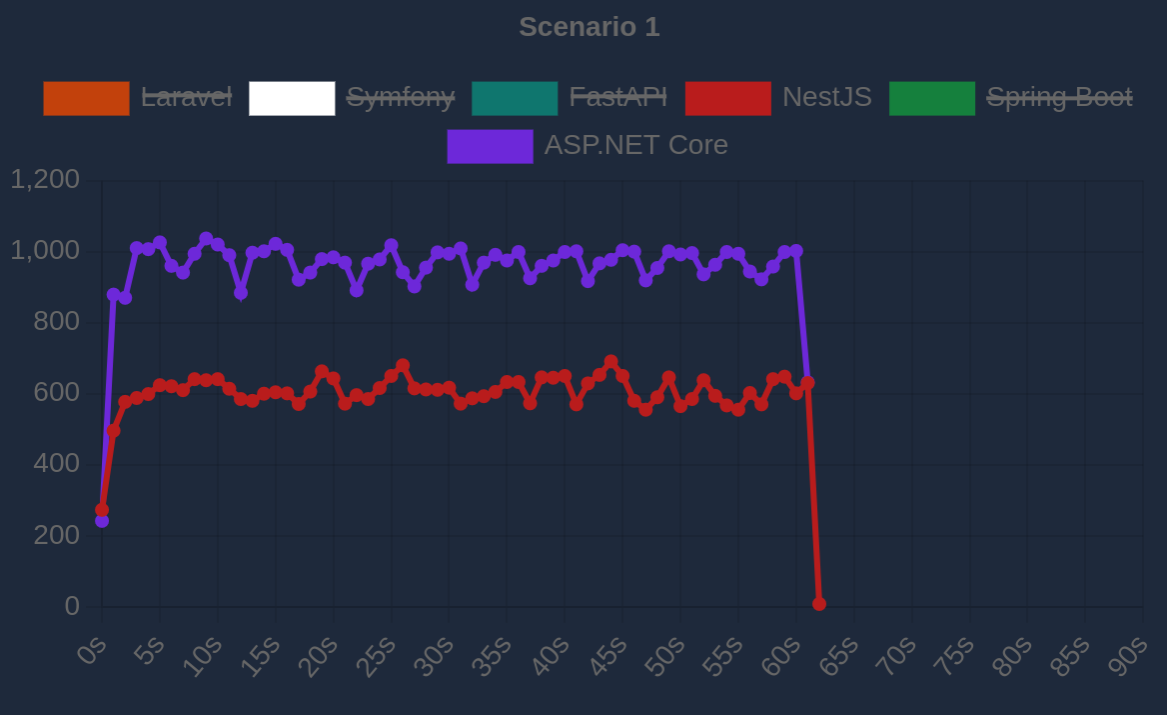
\includegraphics[width=1\linewidth]{rysunki/okla_test_1.png}
	\caption{Zestawienie wyników testów w scenariuszu 1 - źródło: \cite{okami1012024Benchmark}}
	\label{rys:oklatest1}
\end{figure}

W drugim scenariuszu aplikacja była zasypywana dużą ilością zapytań.
Dane były wyciągane z bazy danych, ale były one stosunkowo proste i nie wymagały budowania większych zapytań.
Nacisk został położony na samą obsługę dużej ilości zapytań przez framework.
Wynik testów przedstawiony został na rysunku \ref{rys:oklatest2}.
\begin{figure}[!hb]
	\centering 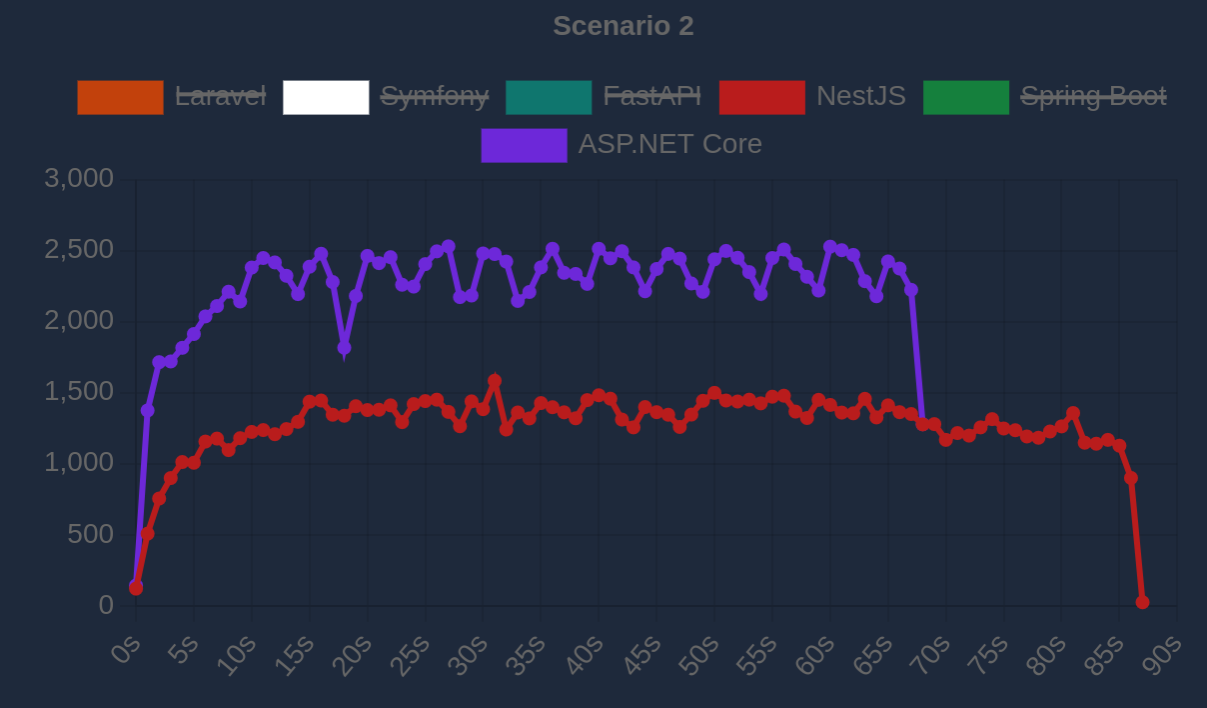
\includegraphics[width=1\linewidth]{rysunki/okla_test_2.png}
	\caption{Zestawienie wyników testów w scenariuszu 2 - źródło: \cite{okami1012024Benchmark}}
	\label{rys:oklatest2}
\end{figure}



Wśród porównywanych frameworków znajdują się .NET oraz NestJS.
Ten drugi konsekwentnie w obu testach wykazał się krótszym czasem odpowiedzi.

